%!TEX root = ../main.tex

\subsection{CAN-bus}
The CAN (Controller Area Network) protocol was originally developed in the 1980's by Bosch.
It is a multi-master network, where each node connects to a common bus.
All nodes are able to broadcast data to all other nodes.
The CAN protocol includes an overhead of 47 bit per message.
The data sent in a message can vary in size from 0 to 8 bytes.
This is described in detail in section~\ref{sub:CanMessageFrame}.
The bus offers 1 Mbit/s on a bus of up to 40 \si{\metre} of length.

\begin{figure}[h!]
	\centering
	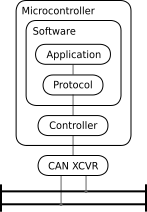
\includegraphics{graphics/canbus_setup}
	\caption{CAN node architecture}
	\label{fig:canbus_setup}
\end{figure}

Some hardware is necessary in order to properly realise a CAN network.
The structure of each node can be seen on figure~\ref{fig:canbus_setup}.
The following paragraphs explain the physical parts of this structure as well as the requirements of the protocol.

\paragraph*{The CAN Bus}~\\
The bus is shown on the bottom of figure~\ref{fig:canbus_setup}.
It is a differential voltage bus.
This means that the value on the bus is determined by the voltage difference of the two wires, rather than the absolute voltage of either wire.
The bus has to be made of twisted pair wires with a characteristic impedance of $\si{120 \ohm}$ and terminated at each end with $\si{120 \ohm}$ resistors.
This increases the EMC of the bus, as inductive noise present on one wire is likely also present on the other, and the noise will then cancel itself out.
That means, that if the bus is broken at any point, no communication will be received, even if the receiving node still has a galvanic connection to the transmitting node.
Alternatively, it is possible to terminate each node, but this greatly reduces transmission speed.\\

\paragraph*{The CAN Transceiver (XCVR)}~\\
As the CAN uses differential voltages, it is not possible to implement directly in the micro controllers.
Typically a micro controller has digital ports putting out either $ 0 \si{\volt}$, or a fixed voltage level defined as "high".
Complementary, it also perceives a voltage level as either low or high. 
As mentioned above, the absolute voltage of either wire of the CAN bus does not matter, but difference in voltage does. 
As there are multiple nodes on the same bus, it is also important for one node to be able to dominate, and the other nodes to know that there is a dominant node. 
This is generally not possible for the micro controller, and it is necessary to use transceivers.
The transceivers translate a Tx voltage signal from the micro controller to the differential CAN signal, and simultaneously translates the bus signal to Rx voltage signal.
The transceivers monitor the bus while transmitting, to see if another node is being dominant, and if that is the case, it will start receiving data.

\paragraph*{The CAN Controller}~\\
This element can be standalone hardware, but it is in many cases built into the micro-controller.
The major advantage of having the controller built into the micro-controller is that it would not otherwise require another protocol, like UART or SPI, to communicate between the microprocessor and controller.
A CAN controller (both standalone and built into a micro controller) has an input and an output FIFO, meaning that the CAN bus communication operates asynchronously. 
It is not a real time network.
This is necessary as there is only one bus and it is likely that there will be a queue of nodes trying to write to the bus.

\paragraph*{Protocol}~\\
\martin{I changed this so that it doesn't mention CANopen, but instead talks about interpreting the base CAN protocol}
The protocol in this case refers to a the interpretation of the CAN protocol.
The design of this protocol will be described in more detail section~\ref{sub:CAN_protocol}. 
Each CAN message comes with some overhead, that among other things can say something about what data the message contains.
This part of the software will interpret this overhead and determine how to handle the data.

CANopen is a widely used protocol made specifically to expand on the usability of CAN.
The SevCon gen4, the motor controller used on the go-kart, utilizes CANopen in its communication.
This makes CANopen a reasonable option to employ generally across the network.
CANopen is, however, quite extensive and implements many features which are not needed in the monitoring system being developed.
Using CANopen would complicate greatly, the task of learning how to add new nodes to the system.
Another option is to design a protocol that fulfills the requirements,
\thomas{Are the requirements of the protocol actually outlined at this point?}
\thomas{At this point it needs to be clear that we want some scalability in the system, enabling us to add up to n (yes n, not 16), nodes. We may need to move figure \ref{fig:analysisnodes} to some other place.}
while still maintaining a simple structure.
As is shown on figure \ref{fig:analysisnodes}, it should be possible to add up to $n$ nodes.
This requirement should be considered in determining the design of the protocol.

\begin{figure}
	\centering
	\includegraphics[width=.75\linewidth]{graphics/analysis_nodes}
	\caption{Overview of the network structure.}
	\label{fig:analysisnodes}
\end{figure}

\thomas{Section describing the requirements of the structure and what requirements that would that result in in terms of the protocol}